\documentclass{beamer}

% Packages.
\usepackage[english]{babel}
\usepackage{graphicx}
\usepackage{amsmath}
\usepackage{amssymb}
\usepackage{comment}
\usepackage[utf8]{inputenc}
\usepackage{lmodern}
\usepackage[T1]{fontenc}
\usepackage[nounderscore]{syntax}
\usepackage{microtype}
\usepackage{nameref}
\usepackage{ulem}

% Styling.
\setlength{\parskip}{1em}
% \usetheme[style=plain,includehead=false,sidebar=true]{uu}
\setlength{\grammarindent}{6.5em}

% Title, subtitle, author and date.
\title{Evolving Levels and Game Agents Using Grammatical Evolution}
\subtitle{Evolutionary Computing 2014}
\author{Bert Massop, Simon Prins, Tom Tervoort}
\date{January 23, 2014}

% Macros.
\makeatletter
\newcommand*{\currentname}{\@currentlabelname}
\makeatother
\newcommand{\paper}[2]{\begin{centering}
\usebeamercolor[fg]{title}\usebeamerfont{title}#1\par
\bigskip\normalsize{}\usebeamercolor[fg]{normal text}\usebeamerfont{normal text}#2\par
\end{centering}}

\begin{document}

% Title page.
\begin{frame}
\titlepage
\end{frame}

\section{Grammatical Evolution}
\subsection{Introduction}
\begin{frame}
\frametitle{Grammatical Evolution}
\begin{itemize}
\item Explained in paper \textit{Grammatical Evolution} by Michael O'Neill et al., 2001.
\item Seeks to evolve sentences in a given context-free grammar.
\item Heavily inspired by biology.
\item Implemented in the GEVA framework.
\end{itemize}
\end{frame}

\subsection{Encoding and Evolution}
\begin{frame}
\frametitle{\currentname}
\begin{itemize}
\item Solutions, or ``chromosomes'', encoded as a finite sequence of (32-bit) natural numbers called ``codons''.
\item Mehcanism:
\begin{itemize}
	\item Move to the next codon for each encountered nonterminal.
	\item Pick a rule to expand it to based on the codon value.
	\item rule index = (codon value) MOD (rule count).
	\item Wrap when reaching the end of the sequence.
	\item Stop when there are no more nonterminals, or a certain depth is reached.
\end{itemize}
\end{itemize}
\begin{itemize}
	\item Different genetic operators can be used.
	\item Here: one-point crossover and mutation by randomizing one codon.
\end{itemize}

\end{frame}

\subsection{Example}
\begin{frame}
\frametitle{\currentname}
\begin{grammar}
<exp>      ::=   \synt{exp} \synt{operator} \synt{exp}  \hfill (0) \hspace{1em}
            \alt \lit*{1.0}    					  		\hfill (1) \hspace{1em}
            \alt \lit*{X}      					  		\hfill (2) \hspace{1em}

<operator> ::=   \lit*{+} 						  		\hfill (0) \hspace{1em}
		    \alt \lit*{-} 						  		\hfill (1) \hspace{1em}
		    \alt \lit*{*} 						  		\hfill (2) \hspace{1em}
		    \alt \lit*{/} 						 		\hfill (3) \hspace{1em}

\end{grammar}

\begin{itemize}

	\only<1>
	{	
		\item Chromosome: \textbf{12 7 33 51 2 44 22 19}
		\item Start with nonterminal <exp>.
		\item 12 MOD 3 = 0, so pick first rule.
	}

	\only<2>
	{	
		\item Chromosome: \textbf{\sout{12} 7 33 51 2 44 22 19}
		\item Sentence: \synt{exp} \synt{operator} \synt{exp}
		\item First expand leftmost subexpression: 7 MOD 3 = 1.
	}

	\only<3>
	{		
		\item Chromosome: \textbf{\sout{12} \sout{7} 33 51 2 44 22 19}
		\item Sentence: \lit*{1.0} \synt{operator} \synt{exp}
		\item Operator is next: 33 MOD 4 = 1.
	}

	\only<4>
	{		
		\item Chromosome: \textbf{\sout{12} \sout{7} \sout{33} 51 2 44 22 19}
		\item Sentence: \lit*{1.0} \lit*{-} \synt{exp}
		\item Remaining subexpression: 51 MOD 3 = 0.
	}

	\only<5>
	{		
		\item Chromosome: \textbf{\sout{12} \sout{7} \sout{33} \sout{51} 2 44 22 19}
		\item Sentence: \lit*{1.0} \lit*{-} (\synt{exp} \synt{operator} \synt{exp})
		\item Continue...
	}

	\only<6>
	{		
		\item Chromosome: \textbf{\sout{12} \sout{7} \sout{33} \sout{51} \sout{2} \sout{44} \sout{22} 19}
		\item Sentence: \lit*{1.0} \lit*{-} (\lit*{X} \lit*{+} \lit*{1.0})
		\item No more nonterminals in sentance, so we are done.
	}

\end{itemize}
\end{frame}

\subsection{Alternative approach}
\begin{frame}
\frametitle{\currentname}

\begin{itemize}
	\item Grammars are trees.
\end{itemize}

\begin{itemize}
	\item Genetic Programming
	\begin{itemize}
		\item Method for evolving tree structures.
		\item Solutions represented as trees in memory.
		\item Crossover: swap branches.
		\item Mutation: change node's contents, while ensuring the tree remains valid.
	\end{itemize}
\end{itemize}

\end{frame}



\section{Ms.\,Pac-Man controller}
\begin{frame}
\paper{Evolving a Ms.\,Pac-Man Controller Using Grammatical Evolution}{E. Galv\'an, J. Swafford, M. O'Neill, and A. Brabazon}
\end{frame}

\subsection{Goal}
\begin{frame}
\frametitle{\currentname}

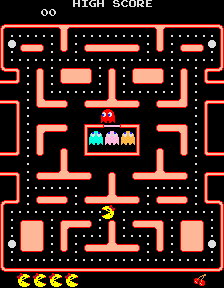
\includegraphics[scale=0.5]{Mspacman.png}
\begin{itemize}
\item Use GE to evolve rules.
\item Rules allow Ms. Pac-Man to maneuver through the maze.
\item Rules maximize score.
\end{itemize}
\end{frame}

\subsection{Experiment setup}
\begin{frame}
\frametitle{\currentname}
Record scores over 100 runs with one life and in one level.
Compare best evolved agent against:
\begin{itemize}
\item Random agent
\item Random non-reverse agent
\item Simple Pill Eater agent
\item Hand-coded agent
\end{itemize}
Against three different ghost teams.
\end{frame}

\subsection{Results}
\begin{frame}
\frametitle{\currentname}
%TODO insert table of scores.

\includegraphics[page=9, trim={3.5cm 10.5cm 3.5cm 3cm}, clip, scale=0.75]{PacMan_GE.pdf}


\end{frame}



\section{Super Mario Bros levels}
\begin{frame}
\paper{Evolving Levels for Super Mario Bros Using Grammatical Evolution}{N. Shaker, M. Nicolau, G. Yannakakis, J. Togelius, and M. O'Neill}
\end{frame}

\subsection{Goal}
\begin{frame}
\frametitle{\currentname}
\begin{itemize}
\item Evolve levels for Infinite Mario Bros using Grammatical Evolution.
\item To provide a framework for analyzing and comparing expressivity ranges of different generators.
\end{itemize}
\end{frame}

\subsection{Experiment setup}
\begin{frame}
\frametitle{\currentname}
Evolve level for Notch's Infinite Mario Bros game.\\
Compare against Notch's level generator and against an adapted version of that generator.\\
Use the following measures to compare them:
\begin{itemize}
\item Linearity
\item Density
\item Leniency
\item Compression Distance
\end{itemize}
\end{frame}

\subsection{Results}
\begin{frame}
\frametitle{\currentname}
\includegraphics[page=5, trim={11cm 15.5cm 1.5cm 8cm}, clip, scale=1.1]{Mario_GE.pdf}
\end{frame}



\section{Discussion}
\subsection{Grammatical Evolution}
\begin{frame}
\frametitle{Discussion}
\begin{itemize}
\item As mentioned, Grammatical Evolution is heavily inspired by biology.
\begin{itemize}
\item \textit{Not necessarily a good thing!}
\item In this case, most references to biological terms are confusing at best.
\end{itemize}
\item Resembling nature is no guarantee for performance.
\item Grammatical Evolution as used here has major flaws.
\end{itemize}
\end{frame}

\begin{frame}
\frametitle{A case against Grammatical Evolution}
\begin{itemize}
\item Simple grammar about kittens\footnote{No kittens were harmed in the production of this presentation.\\} and nuclear missiles
\item Genetic operators as in papers
\item Goal: \textit{make the kitten happy}
\end{itemize}
\end{frame}

\begin{frame}
\frametitle{A simple grammar}
\begin{grammar}
<prog>     ::= \synt{action} \synt{object} \hfill (0) \hspace{1em}
            \alt \lit*{if} \lit*(\synt{object} \lit*{is} \synt{property}\lit*)
              \\\lit*{\{} \synt{prog} \lit*{\}} \hfill (1) \hspace{1em}

<object>   ::= \lit*{nuclear missile} \hfill (0) \hspace{1em}
            \alt \lit*{kitten} \hfill (1) \hspace{1em}

<property> ::= \lit*{dirty} \hfill (0) \hspace{1em}
            \alt \lit*{clean} \hfill (1) \hspace{1em}

<action>   ::= \lit*{clean} \hfill (0) \hspace{1em}
            \alt \lit*{launch} \hfill (1) \hspace{1em}
            \alt \lit*{look at} \hfill (2) \hspace{1em} \par
\end{grammar}
\end{frame}

\begin{frame}
\frametitle{Some sentences}
\framebox{\parbox{19em}{\scriptsize\color{black}
\begin{grammar}
<prog>     ::= \synt{action} \synt{object} \hfill (0) \hspace{1em}
            \alt \lit*{if} \lit*(\synt{object} \lit*{is} \synt{property}\lit*)
              \\\lit*{\{} \synt{prog} \lit*{\}} \hfill (1) \hspace{1em}

<object>   ::= \lit*{nuclear missile} \hfill (0) \hspace{1em}
            \alt \lit*{kitten} \hfill (1) \hspace{1em}

<property> ::= \lit*{dirty} \hfill (0) \hspace{1em}
            \alt \lit*{clean} \hfill (1) \hspace{1em}

<action>   ::= \lit*{clean} \hfill (0) \hspace{1em}
            \alt \lit*{launch} \hfill (1) \hspace{1em}
            \alt \lit*{look at} \hfill (2) \hspace{1em} \par
\end{grammar}}}

\parbox[t][][t]{13em}{\textbf{1 7 4 4 6 3}
\\\texttt{if (kitten is dirty)
\\\{
\\\hspace*{2em}clean kitten
\\\}}
\\\textit{kitten happiness = 9}}
\parbox[t][][t]{13em}{\textbf{8 5 3}
\\\texttt{look at kitten\\\null\\\null\\}
\\\textit{kitten happiness = 7}}
\end{frame}

\begin{frame}
\frametitle{Genetic operator performance}
Let's try 1-point crossover and int-flip mutation.

\framebox{\parbox[t][][t]{13em}{\textbf{1 7 4 4 6 3}
\\\texttt{if (kitten is dirty)
\\\{
\\\hspace*{2em}clean kitten
\\\}}
\\\textit{kitten happiness = 9}}
\parbox[t][][t]{9em}{\textbf{8 5 3}
\\\texttt{look at kitten\\\null\\\null\\}
\\\textit{kitten happiness~=~7}}}
\vfill


\visible<2->{\parbox[t][][t]{13em}{1 \textbf{7 4 4 6 3}
\\\textbf{8} 5 3
\visible<4->{
\\\texttt{launch nuclear missile}
\\\textit{kitten happiness = 0}}}
}
\visible<3->{\parbox[t][][t]{13em}{\sout{1} \textbf{7 4 4 6 3}
\\\textbf{0}
\visible<4->{
\\\texttt{launch nuclear missile}
\\\textit{kitten happiness = 0}}}
}
\end{frame}

\begin{frame}
\frametitle{Luckily\ldots}
\begin{itemize}
\item These problems are operator-dependent.
\item Newer GEVA versions offers more structure-sensitive crossover and mutation operators.
\begin{itemize}
\item Similar to Genetic Programming.
\item \textit{Too bad the authors did not use those!}
\end{itemize}
\end{itemize}
\end{frame}

\subsection{Paper trouble}
\begin{frame}
\frametitle{Not all papers are created equal\dots}
\begin{itemize}
\item Several apparent problems with the papers.
\item Titles are \sout{misleading} not entirely accurate.
\item Experiments cannot be verified
\begin{itemize}
\item Missing parameters
\item Lacking source code
\item Lacking data / results
\end{itemize}
\end{itemize}
\end{frame}

\begin{frame}
\frametitle{Pac-Man trouble}
\begin{itemize}
\item Lacking a solid performance reference point
\begin{itemize}
\item Custom Pac-Man implementation
\item Only one level with one life
\item Weird ghost behaviour
\item \textit{Not even close to Ms.\,Pac-Man}
\end{itemize}
\item Non-repeatable due to lacking information
\end{itemize}
\end{frame}

\begin{frame}
\frametitle{Mario trouble}
\begin{itemize}
\item Pointless fitness function
\item There is nothing wrong with referring to your own work, \\\textit{but don't overdo it}.
\begin{itemize}
\item 15/30 papers referenced have at least one author in common with this work.
\end{itemize}
\visible<2->{\item There is a difference between Super Mario Bros.\ and Notch's Infinite Mario Bros.}
\end{itemize}
\visible<2->{\begin{center}
\includegraphics[height=10em]{notch}
\includegraphics[height=10em]{miyamoto}\end{center}
}
\end{frame}

\begin{frame}
\frametitle{Two optimal levels}
\framebox{
\includegraphics[width=0.9\textwidth]{coin-optimal}}

\framebox{
\includegraphics[width=0.9\textwidth]{goomba-optimal}}
\end{frame}

\begin{frame}
\frametitle{`Wij van WC-eend\ldots'}
\textit{``Procedural Content Generation (PCG) is a field that has
recently emerged and \textbf{proven its potential} for automatically
generating different aspects of game content such as game
rulesets [4], \textcolor<2>{red}{[5]}, maps \textcolor<2>{red}{[6]}, \textcolor<2>{red}{[7]}, levels [8], \textcolor<2>{red}{[9]}, [10], racing
tracks [11], \textcolor<2>{red}{[12]} or even whole games [13], [14]. PCG can
be used both offline, in order to make the game development
process more efficient, and online, to allow the generation of
endless variations of a game, make it infinitely replayable and
adapting its content to the player [15], \textcolor<2>{red}{[16]}. An overview of
the \textbf{state of the art} can be found in \textcolor<2>{red}{[17]}, \textcolor<2>{red}{[18]}.''}
\end{frame}

\section{Conclusions}
\begin{frame}
\frametitle{\currentname}
\begin{itemize}
\item Don't use Grammatical Evolution.
\begin{itemize}
\item Or at least not as described in the O'Neill papers.
\end{itemize}
\item %TODO
\end{itemize}
\end{frame}

\end{document}
